%\documentclass[12pt,a4paper]{article}
\documentclass[letterpaper,12pt,titlepage]{article}

\usepackage{hyperref}
\usepackage{listings}
\usepackage{wasysym}
\usepackage{graphicx}


\hypersetup{
	colorlinks,
	citecolor=black,
	filecolor=black,
	linkcolor=black,
	urlcolor=black
}

% This is a comment
\title{Design Implementation of WellLiv (DIS)}
\author{
  \texttt{Sarahi Pelayo (pelayos)}
  \\[.5ex]
  \texttt{Katherine Jeffrey (jeffreyk)}
  \\[.5ex]
  \texttt{Megan Bigelow (bigelowm)}
  \\[.5ex]
  \texttt{Johnathan Lee (leejohna)}
  \\[.5ex]
  \texttt{Jonathan Rohr (rohrj)}
}

\begin{document}
\maketitle
%UML
\section{UML Class Diagram}
\vspace{50pt}
\hspace*{-1in}
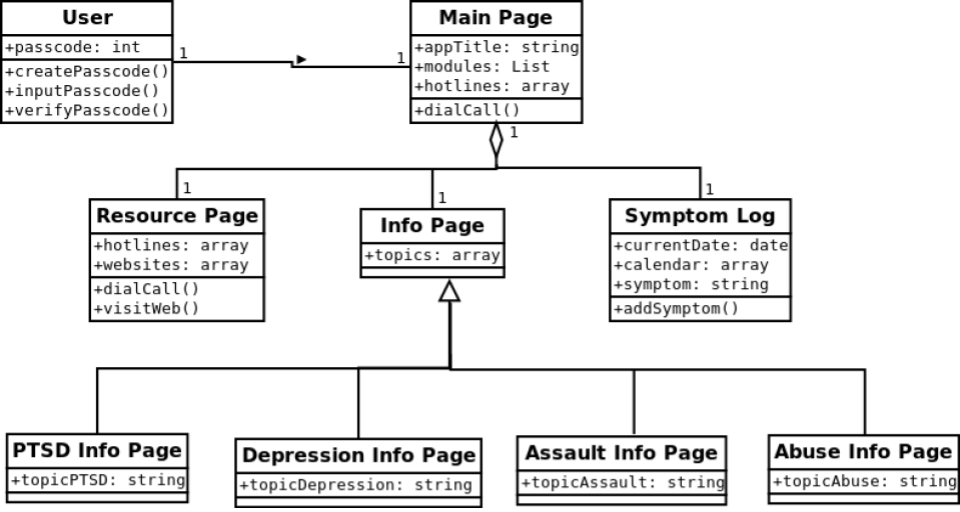
\includegraphics[scale=.55]{UML_Diagram}~\cite{umldia}

\newpage
%Packages
\section{Packages}
\textbf{Package 1:} User class
\noindent
\newline
\newline
The User class contains the attributes and functions associated with the passcode and passcode verification. This class will be one package because it’s only concern is involved with the passcode providing high cohesion. Other packages and code will not be concerning the passcode functionality so this package also has low coupling.
\noindent
\newline
\newline
\textbf{Package 2:} Phone numbers and web links
\noindent
\newline
\newline
The phone numbers and web links package will concern only the necessary code of dialing a phone call and visiting a web link from within the application. This package will have high cohesion as it will only focus on the specific functionality associated with dialing and redirecting to web sites. We expect that this package will also have low coupling which is important when updating any phone numbers or web links.
\noindent
\newline
\newline
\textbf{Package 3:} Symptom Log class
\noindent
\newline
\newline
The Symptom Log class will be a package consisting of the calendar and user symptoms. It will focus on only the functions needed for adding new user symptoms to a data structure that simulates a calendar which stores of the user’s symptom history. The class will have methods for inputting into locations in the data structure that correspond to past dates and well as the current date but not future dates. This package demonstrates high cohesion and low coupling.
\noindent
\newline
\newline
\textbf{Package 4:} Menus class
\noindent
\newline
\newline
The information and resources page both have similar menus. This package will consist of the code needed to create category menus where the user chooses from the three options: PTSD, depression, or sexual assault. Because the output of the application will be based on the choice made by the user at these menus there is high coupling and high cohesion.

\newpage
%Design
\section{Design Patterns}
\textbf{Situation: }Users must enter a passcode and our application will need to verify if the passcode is correct before opening.
\noindent
\newline
\newline
\textbf{Solution: }Strategy Pattern
\noindent
\newline
\newline
When the passcode is entered, the system will need to validate if it is the correct or incorrect code. Strategy would determine which algorithm to initiate in either event. In the case of the correct passcode being entered, the application will open for the user. Otherwise, the login screen will reset and ask the user for their passcode again. This pattern is useful in this situation because there are two events that may occur, depending on the passcode entered by the user, and the correct action needs to be determined before executing.
\noindent
\newline
\newline
\textbf{Situation: }Our application needs to execute events when a user clicks a dial call action or clicks a web link.
\noindent
\newline
\newline
\textbf{Solution:} Observer Pattern
\noindent
\newline
\newline
The observer pattern would be used for the on click events in our application, such as, making phone calls and visiting provided web links from the application. When a user clicks a provided phone number, the observer will be notified of the action and proceed to executing the phone call. Similarly, when a provided web link is clicked, the observer will recognize the action and the user will be directed to the specified website. This pattern is useful since the observer is needed to listen for a specific event and then proceed with the associated action.
\newline
\newline
\noindent
\textbf{Situation: }There are several modules for the user to navigate within our application.
\newline
\newline
\noindent
\textbf{Solution: }Observer Pattern
\newline
\newline
\noindent
The observer pattern would be necessary for identifying actions made in user navigation of our application. We have three modules: Resources, Information and the Symptom Log. Each module sends the user to a specific part of the application with differing attributes and characteristics. The observer will listen for an action made to visit a specific module and proceed to that module.
\newline
\newline
\noindent
\textbf{Situation: }The Symptom Log functionality requires user input of their symptoms on a specified date and storing the input history.
\noindent
\newline
\newline
\textbf{Solution: }Factory Method Pattern
\noindent
\newline
\newline
The Symptom Log consists of a calendar and allows the user to input their specific symptoms for the current date and stores that information. The factory method would be used to create an object for the symptoms that are input each day. This is useful because the symptoms may vary for each date in the calendar and the factory method would create the appropriate object.

%Exception
\section{Exception Handling}
The system’s first instance of exception handling begins with the passcode the user enters to gain access to the program. The systems has error checking for the correctness of the pin entered. An incorrect entry the first time is handled by alerting the user with a message that they made an error and prompts them to re-enter another passcode. While the input stays incorrect the message with continue without granting access until it is correct. 
\newline
\newline
Another part of the system with that deals with an exception is the symptom log. During the normal flow of using the the symptom log feature the user logs their selected symptoms for the current date. In the exception that the user wants to log symptoms for another date our system handles this by changing locations in the data structure which stores the symptoms input to the corresponding date. The user can then enter symptoms for the previous days they want but not for future dates. After they log their symptoms and get their confirmation message of doing so the system returns back to normal after handling the exception. This means the user is returned to the symptom log menu with that current day’s date. 


\newpage
%Meeting
\section{Meeting Report}
\underline{Fourth meeting:} 2/6 in person after class, 5:50pm-6:00pm
\begin{itemize}
\item Members present: Sarahi Pelayo, Katherine Jeffrey, Jonathan Rohr, Megan Bigelow
\item Discussed: Progress on the application done by Katherine. Talked about completing assignment 4.
\item Progress: Assignment 3 was done. Katherine has made an basic outline of the application on android studio and added screenshots of the apps progress to the presentation. It takes input for the passcode, and has menus for resources and information page. The symptom log has been started with a calendar. Sarahi set up the google slides and doc then shared it. Jonathan R. added to the UML class diagram to both.
\item Plans: Complete Assignment 4
\item Customers willing and able to meet.

\end{itemize}
\noindent
\underline{Date:} 2/12 in KEC, 4pm-5pm
\begin{itemize}
\item Progress: Finished assignment 4 and our presentation. Assigned presenters and practiced a bit. Megan completed the design patterns and packages. Johnathan L. worked on the latex file. Sarahi completed the exception handling and helped with the meeting report and packages.
\end{itemize}

\noindent
\textbf{Next Week}
\newline
\newline
Plans and goals:
\noindent
\newline
\newline
Now that the basic shell of the application is implemented the next step is to add functionality. One of the features we will implement next will be the passcode with passcode validation. We will also set up a database. During the week we must also start to add functionality to the rest of the features like the symptom log, information, and the resources page. Progress on the functionality of the application is a priority to stay on track. Less essential part of the plan for the week includes picking a design for the application’s logo and a finalization on choice of color scheme with the current choice being green. Validation of help phone numbers still needs to be done before they are added in.
\newpage

\bibliography{myref}
\bibliographystyle{ieeetr}
\textbf{GitHub Repo:} \url{https://github.com/Rohrj/CS361-001-W2018/tree/Assignment-4/projects/rohrj}

\end{document}